\documentclass[a4paper]{article}
\usepackage[letterpaper,top=2cm,bottom=2cm,left=3cm,right=3cm,marginparwidth=1.75cm]{geometry}
\usepackage[colorlinks=true, allcolors=blue]{hyperref}

\usepackage{wrapfig}
\usepackage{amsthm}
\usepackage{hyperref}
\usepackage{graphicx}
\usepackage{amsfonts}
\usepackage{subcaption}

\title{MPI HW3 | RMA and MPI-IO}
\author{Patryk Drozd}
\begin{document}
\date{}
\maketitle

\section*{Question 1}

	

	\begin{figure}[h!]
		\centering

		\begin{subfigure}[b]{0.32\textwidth}
			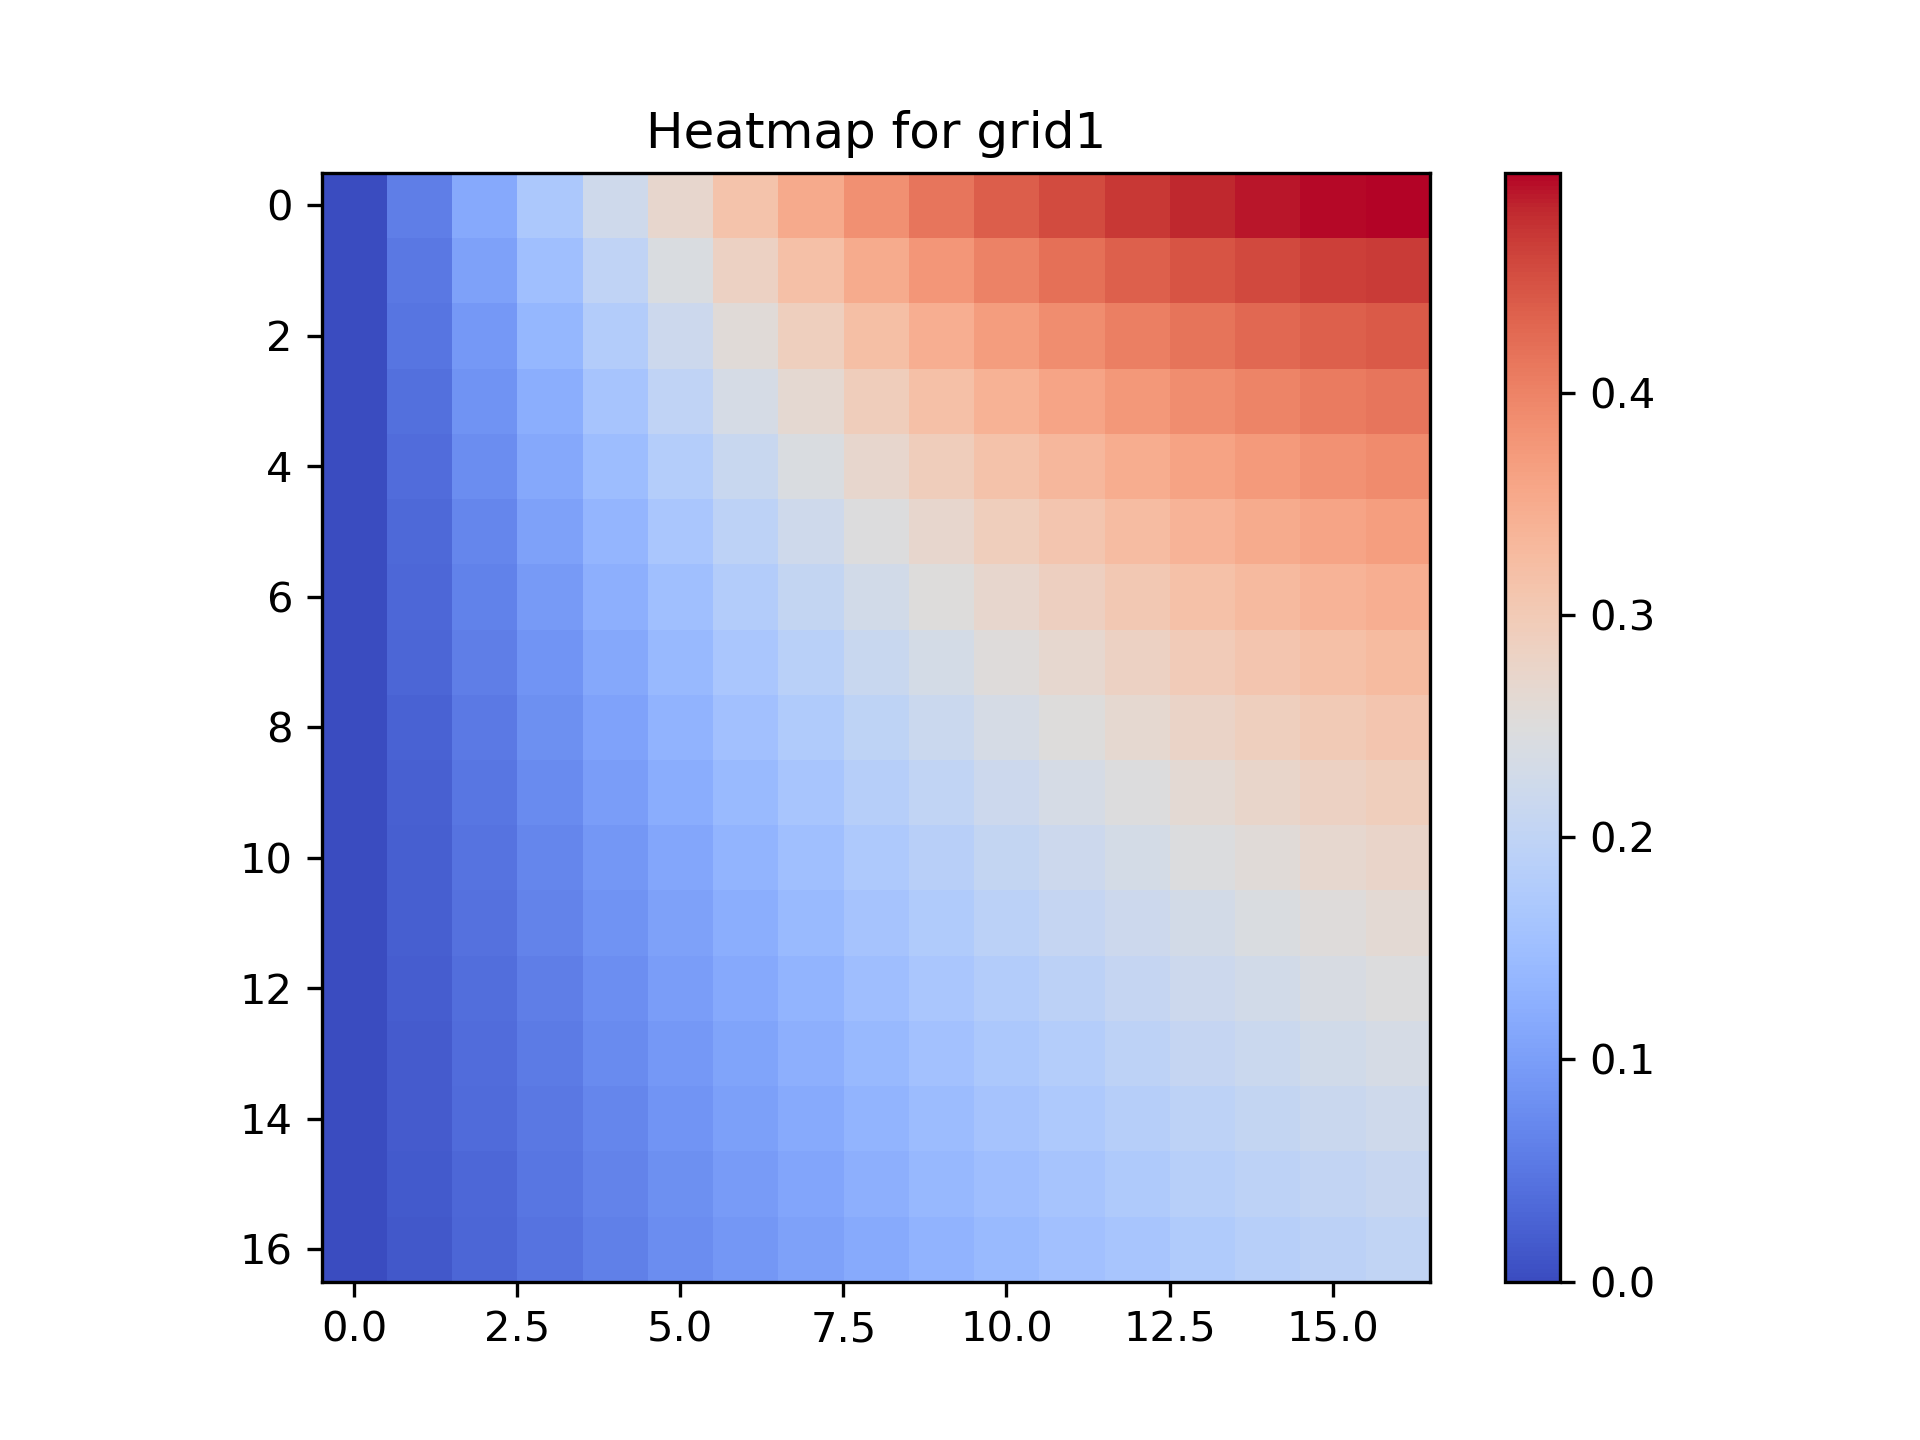
\includegraphics[width=\textwidth]{./../q1/plots/heatmap_plot1.png}
			\caption{Solution for Put and Get with Win\_fence synchronisation.}
			\label{fig:1}
		\end{subfigure}
		\hfill
		\begin{subfigure}[b]{0.32\textwidth}
			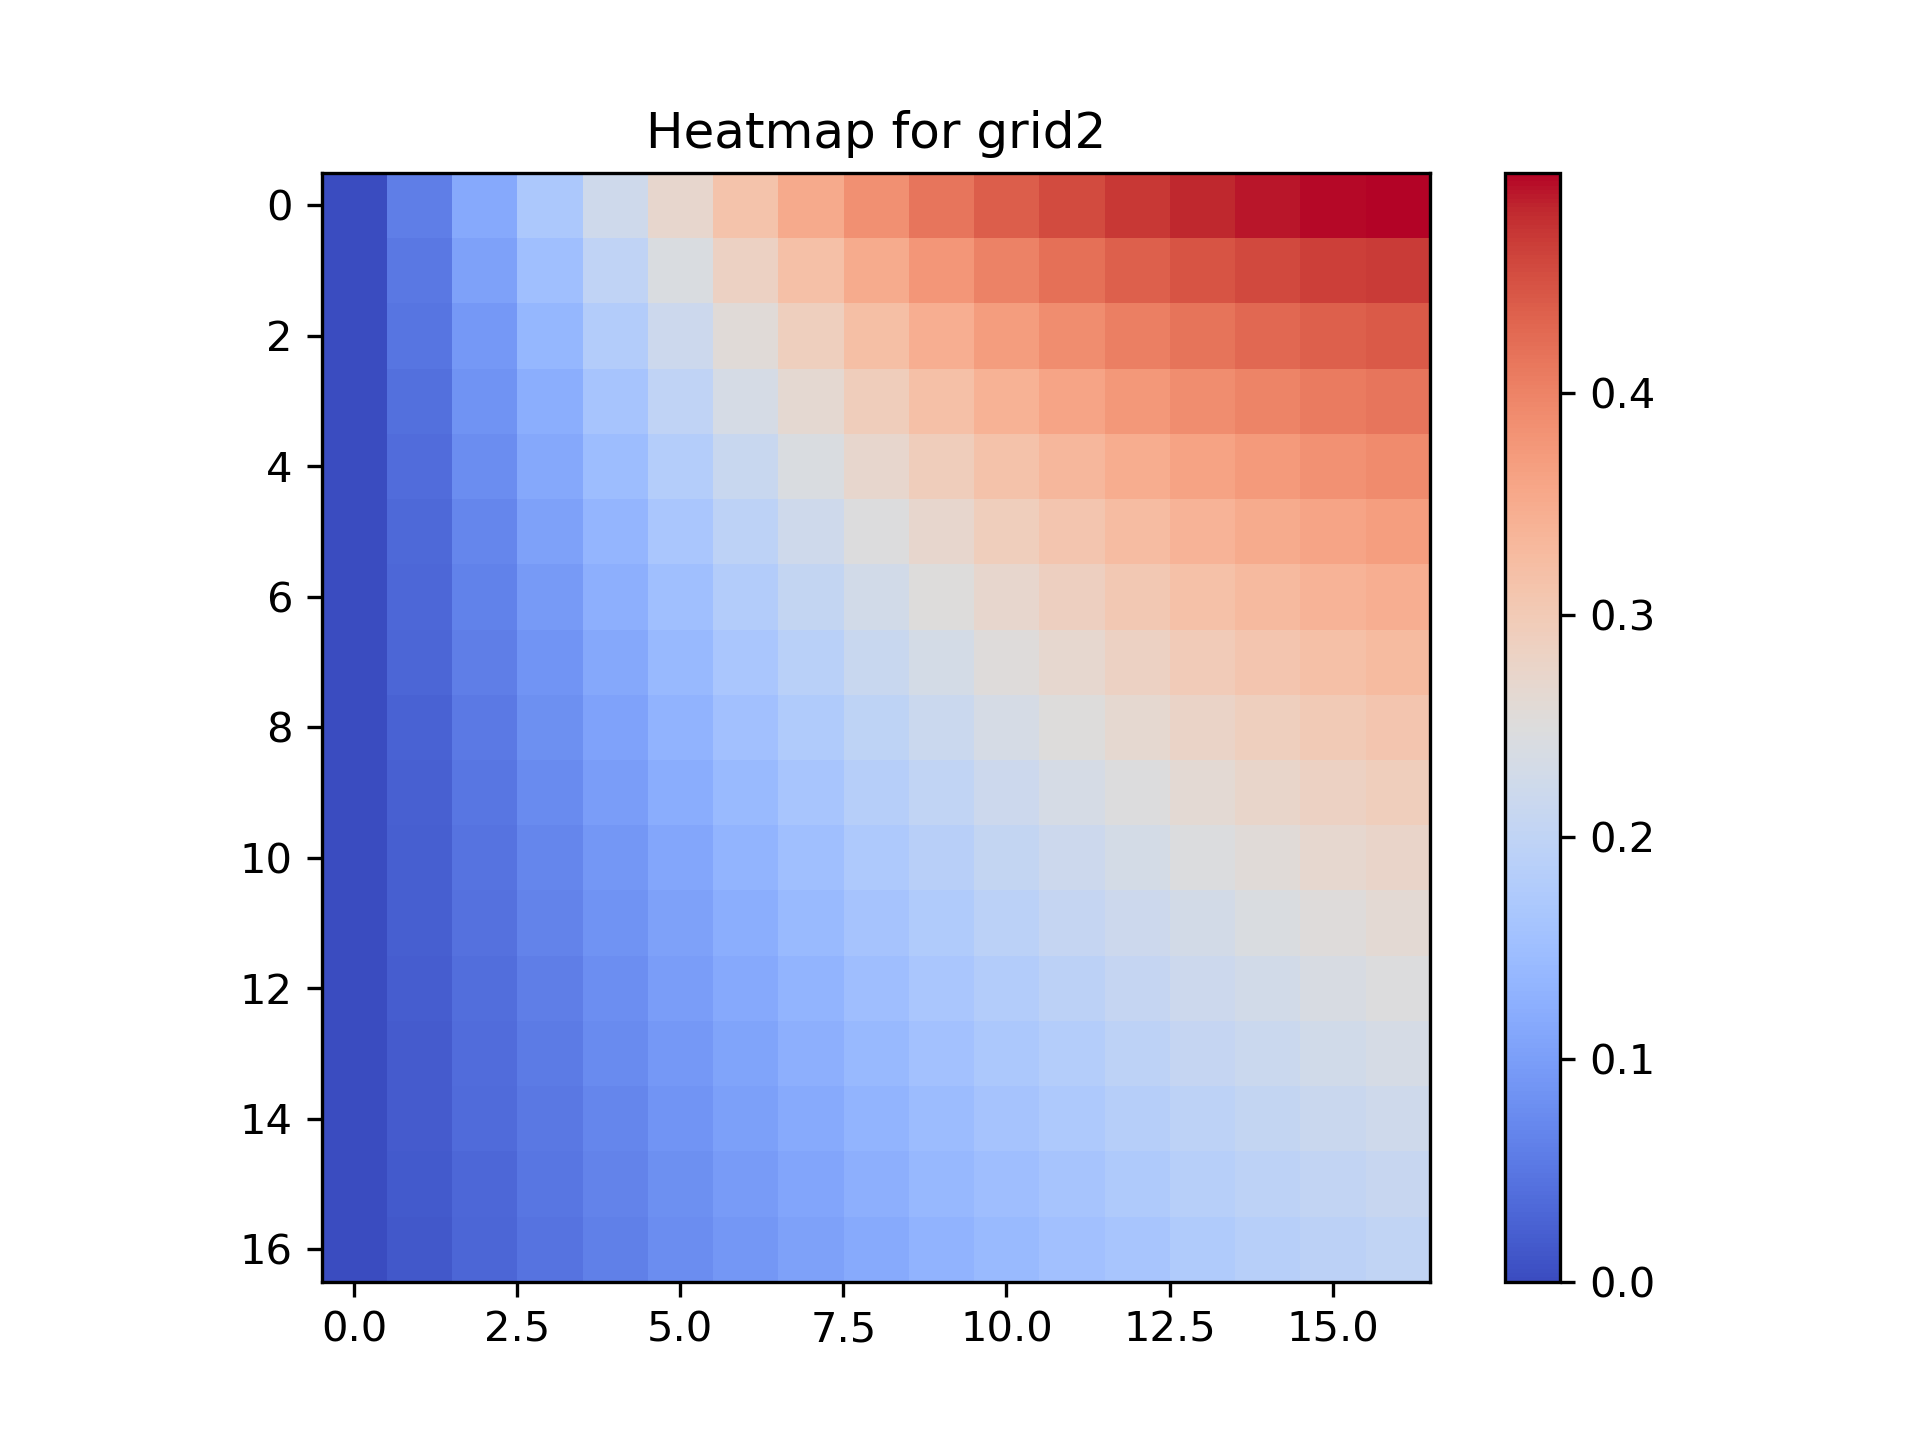
\includegraphics[width=\textwidth]{./../q1/plots/heatmap_plot2.png}
			\caption{Solution for Put and Get with active synchronisation.}
			\label{fig:2}
		\end{subfigure}
		\hfill
		\begin{subfigure}[b]{0.32\textwidth}
			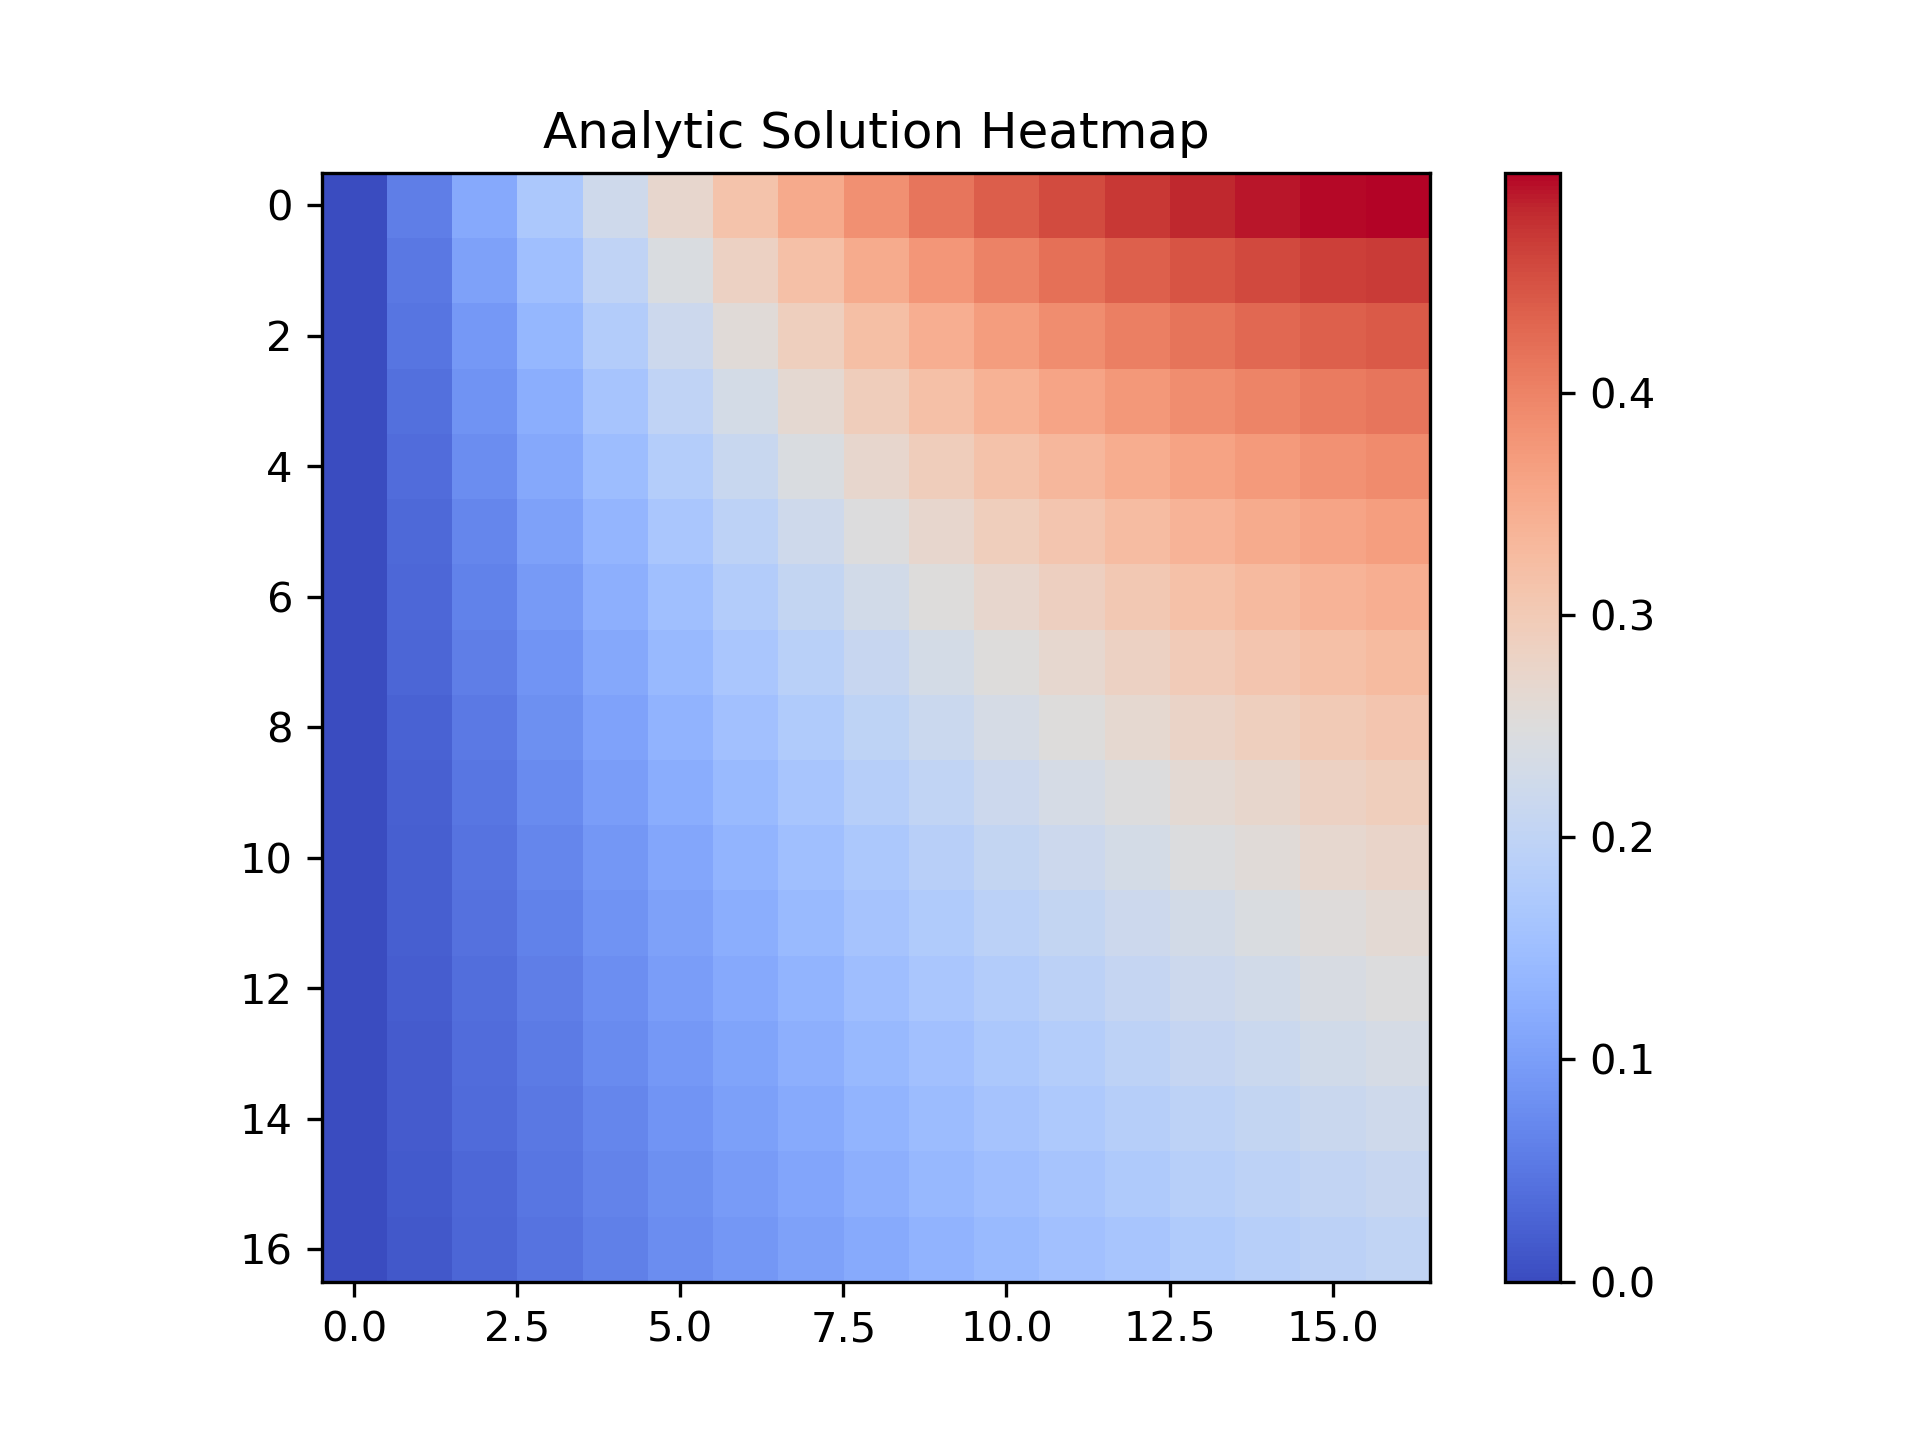
\includegraphics[width=\textwidth]{./../q1/plots/analytic_heatmap_plot.png}
			\caption{Analytic solution of the problem to compare both figures to the left.}
			\label{fig:3}
		\end{subfigure}

		%\caption{Three heatmap plots side by side}
		\label{fig:heatmaps}
	\end{figure}


\section*{Question 2}
		
	Output of this question

	\begin{verbatim}

		Running mpi exercise
		Solution vector: 
		235.0 252.0 282.0 316.0 194.0 226.0 263.0 189.0 210.0 192.0 130.0 
		147.0 163.0 188.0 254.0 245.0 191.0 187.0 197.0 221.0 

		Running python test
		Solution vector:
		[235. 252. 282. 316. 194. 226. 263. 189. 210. 192. 130. 147. 163. 188.
		 254. 245. 191. 187. 197. 221.]

	\end{verbatim}







\bibliographystyle{plain} 
\bibliography{refs} 

\end{document}



